\subsection{Kingdom}
\begin{frame}[t]{Seeking a Kingdom}
\begin{columns}[T, onlytextwidth]
\column{0.5\textwidth}
\Mercury\Retrograde (L1) $\Rightarrow$ \Conjunction\Sun\ $\Rightarrow$ \Sextile\ \Saturn\ (L10) \\
however \\
\Mars\ $\Rightarrow$ \Square\ \Saturn\ (L10) perfects first \\
cutting off the \Sun\ and denying the querent the kingdom \\
\vspace{0.25cm}
And Masha'Allah said the querent would know his hope was lost when \Mars\ perfected its \Square\ to \Saturn \\
\vspace{0.25cm}

Note that the \Moon\ shows the same thing as she first applies to \Mercury, committing her disposition to him and so he hands both his own and her disposition to the the \Sun. And
while  \Mercury\ receives the \Sun, the \Sun\ is not L10 so the matter at hand is not perfected. \\


\column{0.5\textwidth}
\begin{center}
{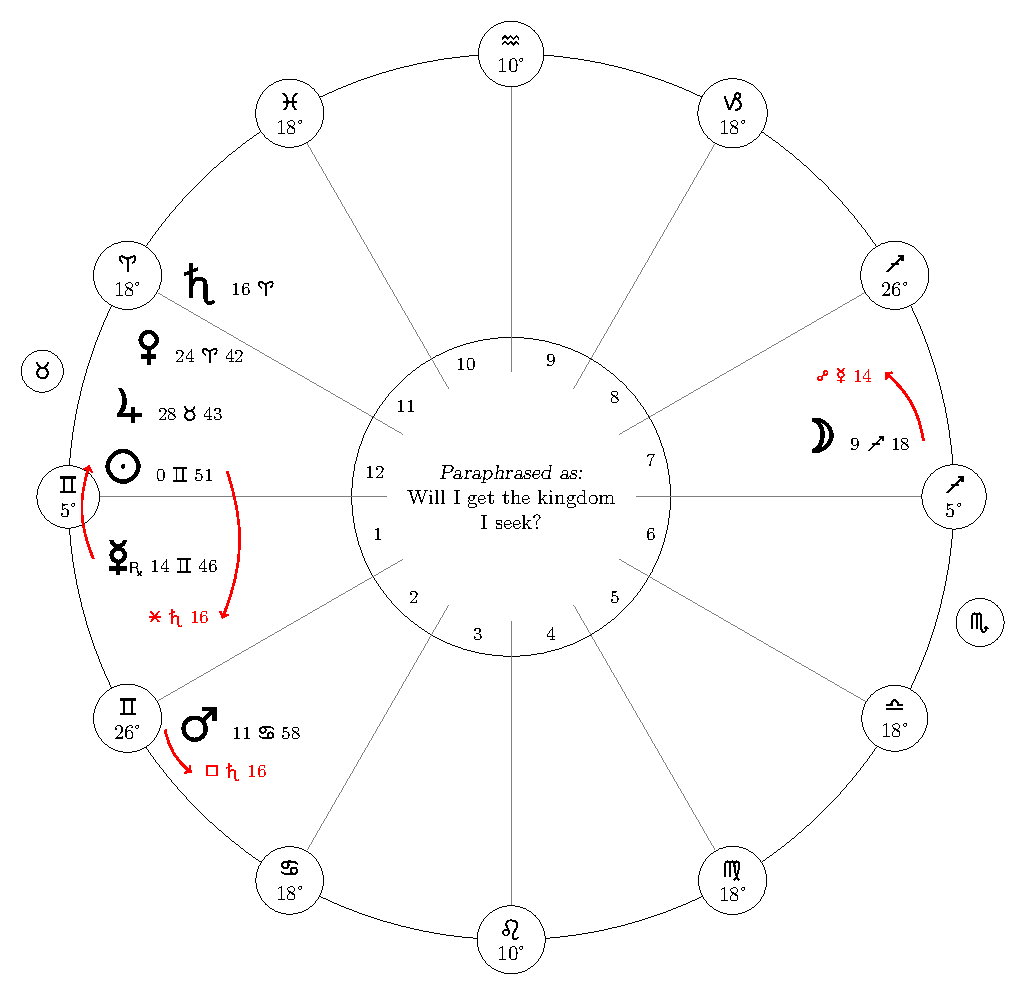
\includegraphics[width=0.9\textwidth]{charts/50-chart-kingdom}} \\
\end{center}
\end{columns}
\end{frame}